\documentclass[11 pt]{beamer}
\usetheme[
	bullet=square,		% Other option: square
	bigpagenumber,		% circled page number on lower right
	topline=true,			% colored bar at the top of the frame 
	shadow= true,			% Shading for beamer blocks
	watermark=BG_lower,	% png file for the watermark
	]{Flip}
%\usepackage{pgfpages}
\setbeameroption{hide notes}

\newcommand{\titleimage}{title}			% Custom title 
\newcommand{\tanedo}{tanedolight}		% Custom author name
\newcommand{\CMSSMDM}{CMSSMDMlight.png}	% light background plot


%%%%%%%%%%
% FONTS %
%%%%%%%%%%
\setbeamerfont{section title}{title}
\setbeamercolor{section title}{titlelike}
%% Default font: lmodern, doesn't require fontspec % solves some default warnings
 %\usepackage[T1]{fontenc} 
 \usepackage[utf8]{inputenc}
 \usepackage[frenchb]{babel}		
%\usepackage{sfmath}		% Sans Serif Math, off by default

%% Protects fonts from Beamer screwing with them
%% http://tex.stackexchange.com/questions/10488/force-computer-modern-in-math-mode
\usefonttheme{professionalfonts}

%\setbeamerfont{title}{family=\fontspec{Gill Sans}}

%%%%%%%%%%%%%%%%%%%%%%%%
% Usual LaTeX Packages %
%%%%%%%%%%%%%%%%%%%%%%%%

\usepackage{amsmath}
\usepackage{amsfonts}
\usepackage{amssymb}
\usepackage{graphicx}
\usepackage{mathrsfs} 			% For Weinberg-esque letters
\usepackage{cancel}				% For "SUSY-breaking" symbol
\usepackage{slashed}            % for slashed characters in math mode
%\usepackage{bbm}                % for \mathbbm{1} (unit matrix)
\usepackage{amsthm}				% For theorem environment
\usepackage{multirow}			% For multi row cells in table
%\usepackage{arydshln} 			% For dashed lines in arrays and tables
\usepackage{tikzfeynman}		% For Feynman diagrams
\usepackage{tikz}
\usepackage{pgfplots}
% \usepackage{subfig}           % for sub figures
% \usepackage{young}			% For Young Tableaux
% \usepackage{xspace}			% For spacing after commands
% \usepackage{wrapfig}			% for Text wrap around figures
% \usepackage{framed}
\usepackage{graphics}

\graphicspath{{images/}}	% Put all images in this directory. Avoids clutter.


\usetikzlibrary{backgrounds}
\usetikzlibrary{mindmap,trees}	% For mind map
% http://www.texample.net/tikz/examples/computer-science-mindmap/


% SOME COMMANDS THAT I FIND HANDY
% \renewcommand{\tilde}{\widetilde} % dinky tildes look silly, dosn't work with fontspec
\newcommand{\comment}[1]{\textcolor{comment}{\footnotesize{#1}\normalsize}} % comment mild
\newcommand{\Comment}[1]{\textcolor{Comment}{\footnotesize{#1}\normalsize}} % comment bold
\newcommand{\COMMENT}[1]{\textcolor{COMMENT}{\footnotesize{#1}\normalsize}} % comment crazy bold
\newcommand{\Alert}[1]{\textcolor{Alert}{#1}} % louder alert
\newcommand{\ALERT}[1]{\textcolor{ALERT}{#1}} % loudest alert
%% "\alert" is already a beamer pre-defined



\author[Password team]{Céline Caldini-Queiros, Bruno Deprés, Lise-Marie Imbert-Gérard, Maryna Kachanovska (with Olivier Lafitte and Remi Sart)}
\title[Password]{Password projects}		
\institute{Cemracs 2014}
\date{27.08.2014}
\newcommand{\blue}[1]{\textcolor{beaubleu!70!black}{#1}}
\usefonttheme[onlysmall]{structurebold}

\usepackage{boiboite2}
\usepackage{marenewcommand}
\usepackage{subfigure}
\begin{document}

%%%%%%%%%%%%%%%%%%%%%%%%
% Additional  settings %
%%%%%%%%%%%%%%%%%%%%%%%%

%% To use external nodes; http://www.texample.net/tikz/examples/beamer-arrows/
\tikzstyle{every picture}+=[remember picture]


%%%%%%%%%%%%%%%%%%%%%%%%
% Actual content below %
%%%%%%%%%%%%%%%%%%%%%%%%

%% It's much nicer to have all the content in a separate file
% DO NOT COMPILE THIS FILE DIRECTLY!
% This is included by the the driver file (FlipBeamerTemplate.tex).

%{ %% This is a total kludge for a fancy title page background
%\setbeamertemplate{sidebar right}
 {\setbeamertemplate{sidebar right}{\llap{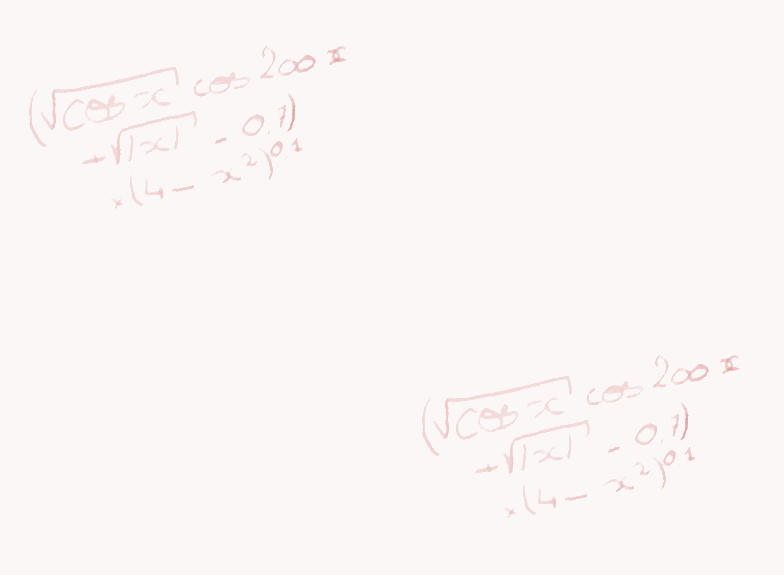
\includegraphics[width=\paperwidth,height=\paperheight]{BG_upper}}}
\begin{frame}[c]%{\phantom{title page}} 
% The \phantom{title page} is a kludge to get the red bar on top
% \titlepage
\begin{center}
	% \includegraphics[width=7cm]{WarpedPenguinsReturn}
%\vspace*{-2cm}
	\begin{tikzpicture}%[show background grid] %% Use grid for positioning, then turn off
		\node[inner sep=10pt,anchor =north west] (title) 
			{ \includegraphics[width=7cm]{\titleimage} };
			 \node (title) at (0.5,-2.5) {};
	\end{tikzpicture}
	\quad

	% \includegraphics[width=7cm]{\titleimage} 
	%\vspace*{1cm}
	\tiny{Céline Caldini-Queiros, Bruno Després, Lise-Marie Imbert-Gérard, Maryna Kachanovska\\ (with Olivier Lafitte and Remi Sart)}
	\vspace{.5em}
	
	\footnotesize\textcolor{brunfonce}{08.04.2014}
%	\texttt{[arXiv:1234.5678]}
	\vspace{1cm}
%	

\end{center}
\end{frame}}
\begin{frame}{Model}
 \begin{minipage}{0.45\linewidth}
 \begin{figure}
       		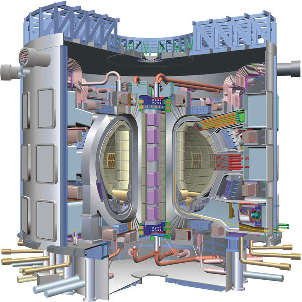
\includegraphics[scale = 0.7]{./images/ITER_cut}
       	\caption{ITER}
     	 \end{figure} 
\end{minipage}
\hfill
\begin{minipage}{0.45\linewidth}
 \begin{figure}
       		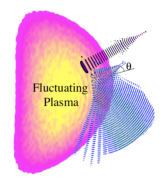
\includegraphics[scale = 1.2]{./images/antenne}
       		\caption{waves}
     	 \end{figure} 
\end{minipage}
\begin{block}{Equations : Maxwell-Newton}
\[
\begin{cases}
&-\frac{1}{c^2}\partial_t E + \nabla \wedge B = \mu_0 J \hspace{3cm} J = e N_e u_e\\
&\partial_t B + \nabla \wedge E  = 0	\\
&m_e \partial_t u_e  =  -e(E + u_e \wedge B_0 ) - m_e \nu u_e
\end{cases}
\]
\end{block}


\end{frame}
\begin{frame}{Some references}
\begin{itemize}
\item Décomposition de domaines pour la simulation "full wave" dans un plasma froid, T. Hattori (thesis) \\ 
\item Analyse mathématique et numérique de problèmes d’ondes apparaissant dans les plasmas
magnétiques, L.-M. Imbert-Gérard (thesis)\\ 
\item Hybrid resonance of Maxwell's equations in slab geometry, B.Després, L.M. Imbert-Gérard and R. Weder, in JMPA\\ 
\item  Stable coupling of the Yee scheme with a linear current model, F. Da Silva, M. Campos-Pinto, B. Després, S. Heuraux, HAL preprint 2014. \\ 
\item Full-wave modeling of the O-X mode conversion in the Pegasus Toroidal Experiment, A. Kohn, J. Jacquot, M.W. Bongard, S. Gallian, E.T. Hinson and F.A. Volpe, arXiv:1104.0743 [physics.plasm-ph](2011).
\end{itemize}
\end{frame}
\begin{frame}{Frequency domain study}
In 1D : $\partial_t = \imath \theta$. Unknowns : $\ubf =(E_1,E_2) = (E_x,E_y)$


\alert{Variational formulation :}
\[
\begin{array}{l}
\displaystyle \int_{-L}^H (E_2' -\imath\theta E_1)\overline{(\tilde E_2' -\imath \theta \tilde E_1)} - \int_{-L}^H (\eps_0 +\imath\nu Id) \E \cdot \overline{\tilde \E}
\\ \displaystyle  - \imath \sqrt{\alpha(-L)} E_2 (-L) \tilde E_2 (-L) = -g_{inc} (-L) \overline{( \tilde E_2(-L) )} 
\end{array}
\]
\[
a(\ubf,\vbf) = a_1 (\ubf,\vbf) +\imath a_2(\ubf,\vbf)\  \text{ and } \  l(\vbf) = -g_{inc} (-L) \overline{(v_2(-L) )} 
\]
\[
\left\{\begin{array}{l}
a_1(\ubf,\vbf) = \int_{-L}^H (u_2' -\imath\theta u_1)\overline{(v_2' -\imath \theta v_1)} - \int_{-L}^H \eps_0 \ubf\cdot \overline{\vbf}, 
\\ a_2(\ubf,\vbf) = -\nu \int_{-L}^H  \ubf\cdot \overline{\vbf} -  \sqrt{\alpha(-L)} u_2 (-L) \overline{v_2 (-L)} , 
\end{array}\right.
\]
where $a_1= a_1^*$ and $a_2=a_2^*$ are hermitian.
\end{frame}
\begin{frame}{Frequency domain study}
\[
|a(\ubf,\ubf)| \geq \frac{1}{4} \sqrt{\frac{\nu}{\heps + \theta^2}}\|u_2'\|^2_{L^2} +  \frac{\nu}{4} \|\ubf\|_{L^2}^2,
\]
\begin{block}{}
\[
|a(u,u)| \geq \min\left(\frac{1}{4} \frac{\sqrt{\alpha(-L)}}{|\Omega|} , \frac{1}{16}\frac{\sqrt{\frac{\nu}{\heps + \theta^2}}}{|\Omega|^2}\right) \|u\|^2_{L^2}
\]
\end{block}
\end{frame}

\begin{frame}{Simulation in frequency domain}
\ALERT{Matlab code, $P^1$ FEM}

\ \\

 \begin{minipage}{0.45\linewidth}
\begin{figure}
	\begin{center}
       	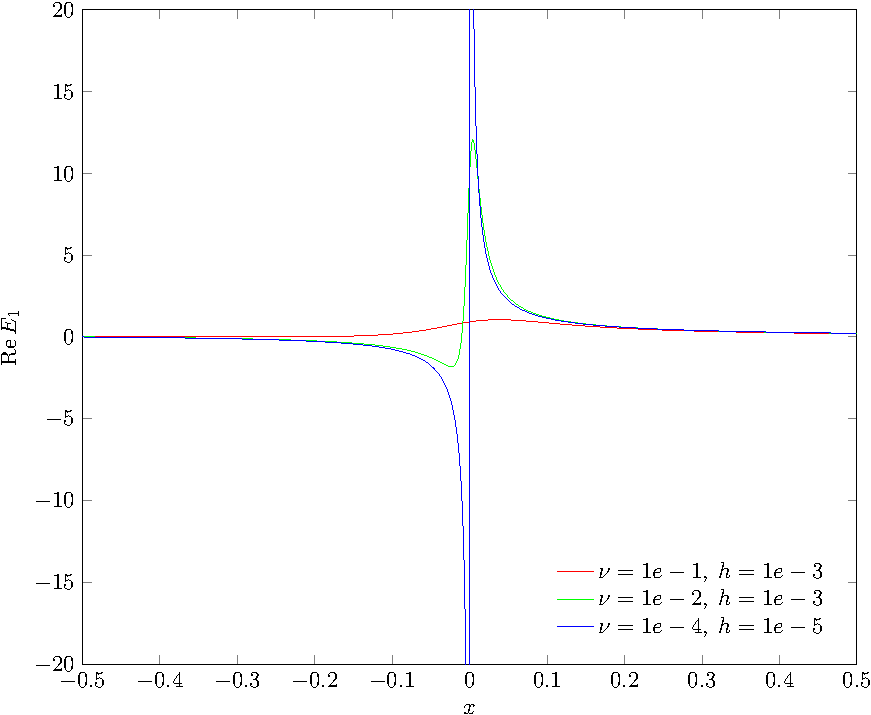
\includegraphics[width = 0.9\textwidth]{./images/picture2}
       	\caption{Convergence $E_x^\nu(x)$}
    \end{center}
\end{figure} 
\end{minipage}
\hfill
\begin{minipage}{0.45\linewidth}
	\begin{figure}
\begin{center}
       	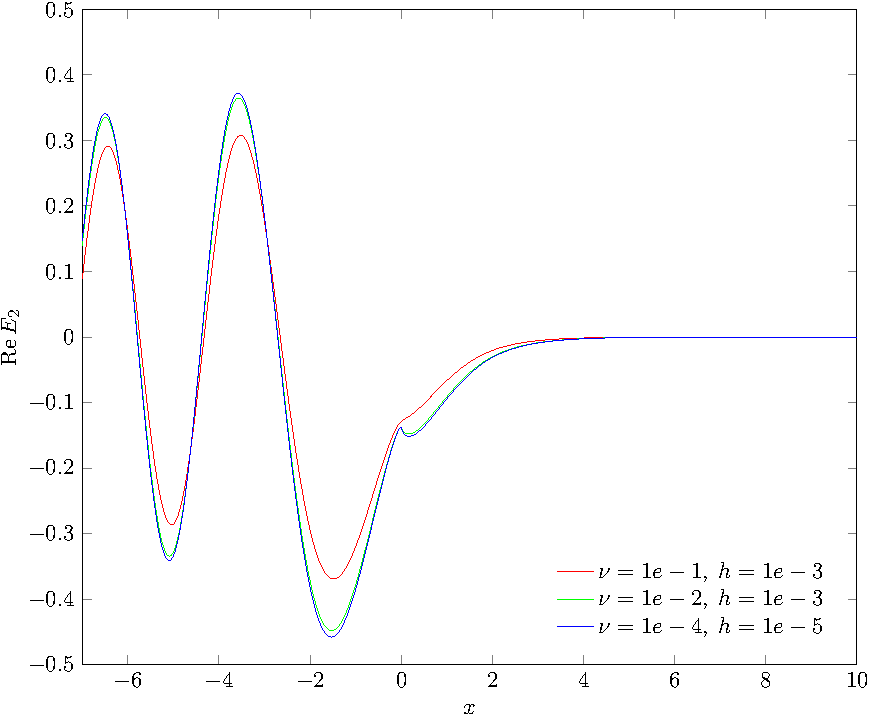
\includegraphics[width = 0.9\textwidth]{./images/pics3}
       	\caption{Convergence $E^\nu_y(x)$}
    \end{center}
\end{figure} 
\end{minipage}
\[
E_x^\nu \approx \frac{c}{x + \imath \nu}
\]

\end{frame}
\begin{frame}
\begin{figure}[ht]
\subfigure[Convergence rates]{
    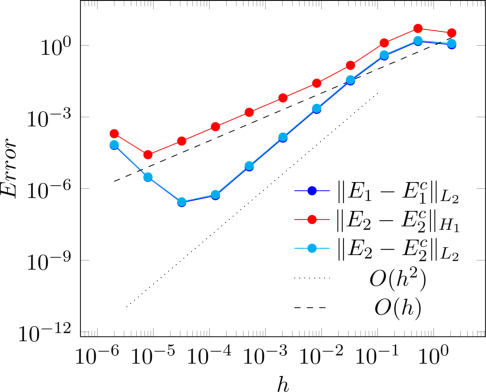
\includegraphics[width=0.4\textwidth]{./images/fig1}
  }
  \subfigure[The $L_2$ error of $E_x(x)$]{
    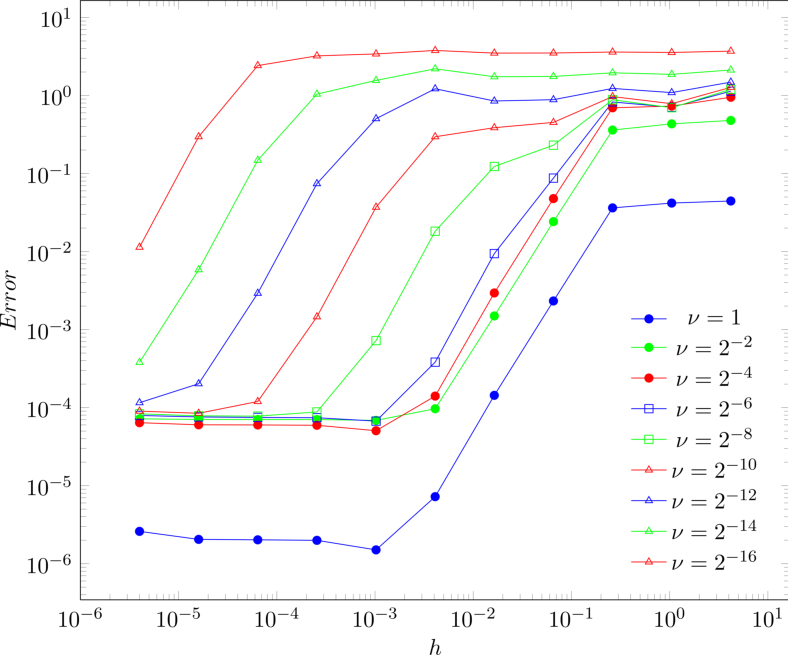
\includegraphics[width=0.4\textwidth]{./images/fig2}
  }
  
  \subfigure[The $L_2$ error of $E_y(x)$]{
    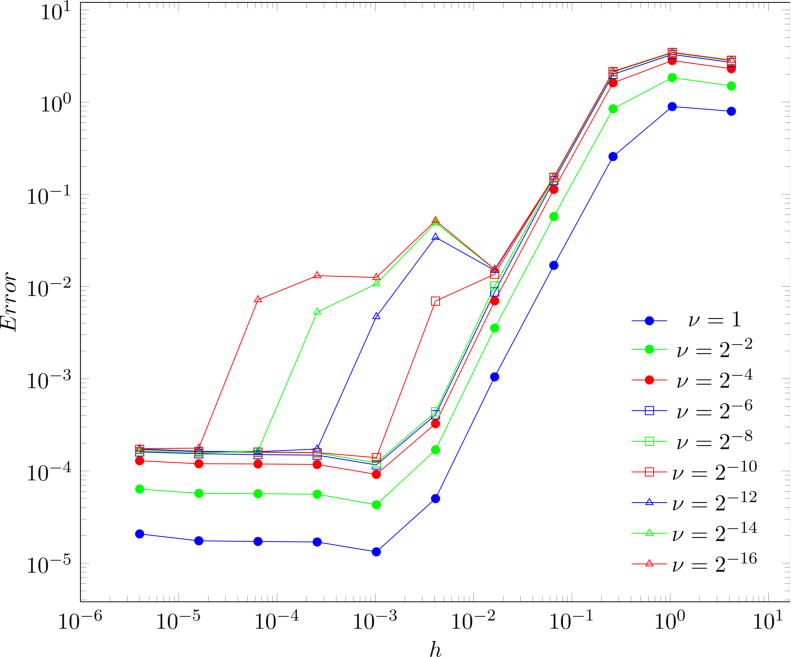
\includegraphics[width=0.4\textwidth]{./images/fig3}
  }
  \subfigure[The dependance of $h_\veps$ in $\nu$]{
    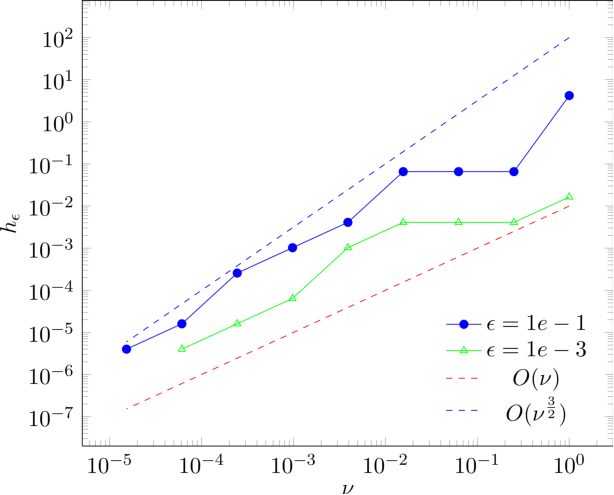
\includegraphics[width=0.4\textwidth]{./images/fig4}
  }
  
\end{figure}
\end{frame}

\begin{frame}{Time dependant problem}
\[
\begin{cases}
- \veps_0 \partial_t E_x = e N_e u_x \\
- \veps_0 \partial_t E_y - \partial_x E_y = 0 e N_e u_y \\
\partial_t H_z + \partial_x E_y = 0 \\
m_e \partial_t u_x = e (E_x + u_y B_0) - \nu m_e u_x
m_e \partial_t u_y = e (E_x - u_x B_0) - \nu m_e u_y
\end{cases}
\]

\alert{Finite difference, 1D energy conservative scheme\footnote{ Stable coupling of the Yee scheme with a linear current model, F. Da Silva, M. Campos-Pinto, B. Després, S. Heuraux, HAL preprint 2014}}


\end{frame}
 {\setbeamertemplate{sidebar right}{\llap{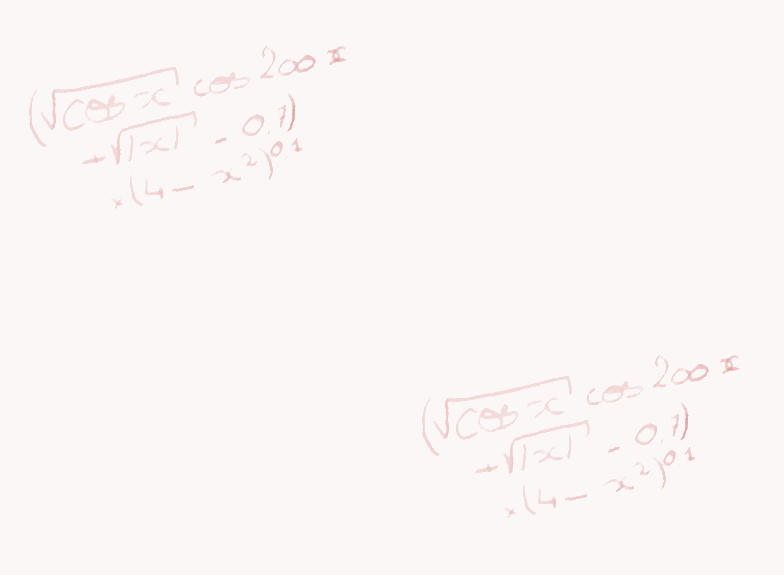
\includegraphics[width=\paperwidth,height=\paperheight]{BG_upper}}}
\begin{frame}
\begin{center}
\textcolor{lightred}{\scalebox{2}{Thank you for your attention !}}
\end{center}
\end{frame}}



% \begin{frame}{test}
% 	Main text still in Gill Sans
% 	$$\frac{f}{f^4}$$
% 	
% 	But math is now different
% 	\Large
% 	$$\frac{f^2}{f^4}$$
% \end{frame}


\end{document}
